\documentclass{beamer}

\usepackage{amsmath}
\usepackage{amssymb}
\usepackage{accents}
\usepackage{graphicx}
\usepackage{adjustbox}
\usepackage{color}
\usepackage{float}
\usepackage{array}
\usepackage{bm}
\usepackage[titlenumbered,longend,ruled,linesnumbered]{algorithm2e}
\usepackage{tikz}
\usetikzlibrary{fit,shapes,arrows,automata}
\usepackage{3dplot}
\tdplotsetmaincoords{50}{105} % viewing angle
\input{tikz-parallelepiped.inc}
\input{spheres.inc}
\usepackage{tabto}

\title{Probabilistic Discovery of Articulated Object Kinematics Using Trajectory Matching with a pseudo-Riemannian Metric on $SE(3)$}
\author{Alex Burka}
\date{March 20, 2013}

\newcommand{\mat}[2]{\ensuremath{\left[\begin{array}{#1}#2\end{array}\right]}}
\newcommand{\deriv}[2]{\ensuremath{\frac{d#1}{d#2}}}
\newcommand{\pderiv}[2]{\ensuremath{\frac{\partial #1}{\partial #2}}}
\newcommand{\dsum}{\ensuremath{\displaystyle\sum}}

% random helper commands
\DeclareMathOperator*{\argmin}{argmin}
\DeclareMathOperator*{\argmax}{argmax}
\DeclareMathOperator*{\proj}{proj}
\DeclareMathSymbol{\widehatsym}{\mathord}{largesymbols}{"62}
\newcommand\lowerwidehatsym{%
  \text{\smash{\raisebox{-1.3ex}{%
    $\widehatsym$}}}}
\newcommand\bowler[1]{%
  \mathchoice
    {\accentset{\displaystyle\lowerwidehatsym}{#1}}
    {\accentset{\textstyle\lowerwidehatsym}{#1}}
    {\accentset{\scriptstyle\lowerwidehatsym}{#1}}
    {\accentset{\scriptscriptstyle\lowerwidehatsym}{#1}}
}
\newcommand{\overbar}[1]{\mkern 4mu\overline{\mkern-4mu#1\mkern-4mu}\mkern 4mu}

% notation
\def\change{ {\mathsmaller\Delta} }
\def\xmat{\uppercase}    \def\xmatstr{in uppercase}
\def\xvec{\vec}          \def\xvecstr{with an arrow}
\def\xse{\bar}            \def\xsestr{with a bar}

\begin{document}

    \TabPositions{4cm}

    \frame{\titlepage}

    \begin{frame}{Motivation}{OR: a map of the rabbit hole}
      \fontsize{8pt}{10pt}\selectfont
      \begin{itemize}[<+->]
        \pause
        \item End goal: robot interacts with real world object and learns a kinematic tree
        \item Input: feature trajectories \tab $x_i(t) \in SE(3)$
        \item Output: kinematic tree \tab $Rigid(1, Prismatic(2, Revolute(3, 4)))$
        \item Key subproblem: fit several candidate joint models to a set of feature trajectories, and decide on the best model
        \item Sticking point 1: how do we compare the observed and predicted trajectories of a feature? We need to be able to compare elements of $SE(3)$.
        \item Sticking point 2: how do we determine which sub-objects are connected?
      \end{itemize}
      \vspace{-.25in}
      \begin{figure}[h]
        \centering
        \tikzstyle{node} = [draw, ellipse, font=\scriptsize]
        \begin{tikzpicture}
          \uncover<4->{
            \node (seat) [node, accepting] at (-7.5,1) {seat};
            \node (backrest) [node, right of=seat, node distance=2cm] {backrest};
            \node (base) [node, below of=seat, anchor=west, node distance=1cm] {base};
            \node (wheel2) [node, below of=base, font=\tiny, node distance=1cm] {wheel};
            \node (wheel1) [node, left of=wheel2, font=\tiny, node distance=1cm] {wheel};
            \node (wheel3) [node, right of=wheel2, font=\tiny, node distance=1cm] {wheel};

            \draw [font=\tiny, ->] (seat) to [above] node {R} (backrest);
            \draw [font=\tiny, ->] (seat) to [left] node {P+R} (base);
            \draw [font=\tiny, ->] (base) to [bend right, above] node {R} (wheel1);
            \draw [font=\tiny, ->] (base) to [right] node {R} (wheel2);
            \draw [font=\tiny, ->] (base) to [bend left, above] node {R} (wheel3);
            \draw [font=\tiny, -, dashed] (wheel1) to [bend right] node {} (wheel2);
            \draw [font=\tiny, -, dashed] (wheel2) to [bend right] node {} (wheel3);
          }

          \uncover<2->{
            \node (pr2) {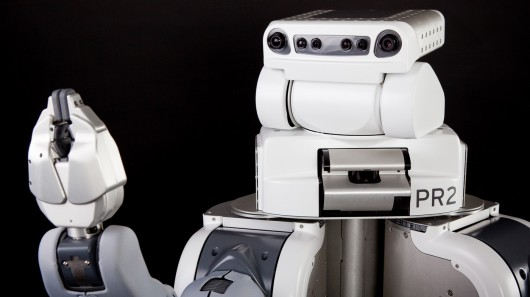
\includegraphics[scale=.3]{pres_img/pr2robot.jpeg}};
            \node (bop) at (pr2.north west) {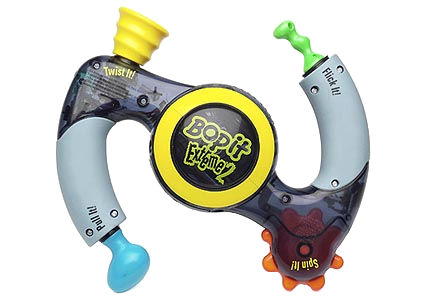
\includegraphics[scale=.2]{pres_img/bopit.png}};
          }
        \end{tikzpicture}
      \end{figure}
    \end{frame}

    \begin{frame}{Literature Review}
      \begin{columns}[t]
        \column{0.71\textwidth}
        \begin{itemize}[<+->]
          \small
          \vspace{-.2in}
          \pause
          \item Interactive Perception (Katz et al 2008, 2012)
            \begin{itemize}
              \scriptsize
              %\vspace{-.15in}
              \item Perception and action are not as decoupled as roboticists like to pretend
              \item Tracking: optical flow, Lucas-Kanade registration, SIFT features
              \item Segmentation: weighted max-flow/min-cut (?)
              \item Fitting: ad-hoc rigid/prismatic/revolute
            \end{itemize}
          \item Motion subspaces (Yan \& Pollefeys 2006)
            \begin{itemize}
              \scriptsize
              \item Joints restrict the motion of object parts to intersecting subspaces of $SE(3)$
              \item Tracking/segmentation: bypassed (input is trajectories)
              \item Fitting: estimate subspace of each feature, build graph using the principle angles between all subspaces, then minimum spanning tree
            \end{itemize}
          \item Probabilistic approach (Sturm et al 2011)
            \begin{itemize}
              \scriptsize
              \item Bayesian treatment of the trajectory matching problem
              \item Main inspiration for the current paper
              \item Tracking/segmentation: augmented reality markers
              \item Fitting: nonlinear optimization using kinematics, then minimum spanning tree on BIC
            \end{itemize}
        \end{itemize}

        \column{0.5\textwidth}
        \begin{figure}[h]
          \vspace{-.5in}
          \centering
          \uncover<2->{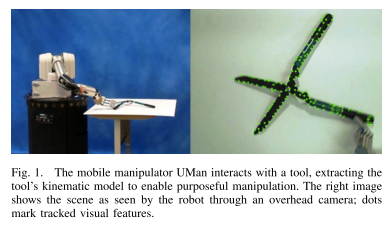
\includegraphics[height=0.3\textheight]{pres_img/katz.png}}
          \linebreak
          \uncover<7->{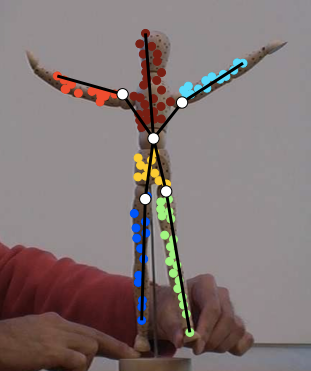
\includegraphics[height=0.3\textheight]{pres_img/yan.png}}
          \linebreak
          \uncover<11->{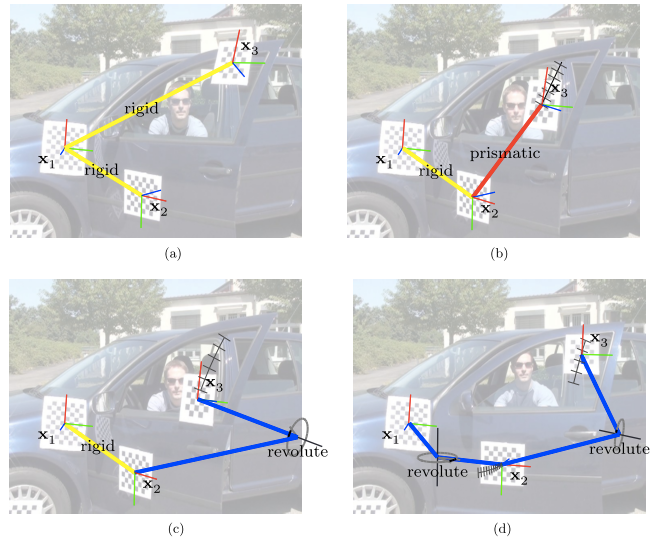
\includegraphics[height=0.3\textheight]{pres_img/sturm.png}}
        \end{figure}
      \end{columns}
    \end{frame}

    \begin{frame}{Probabilistic Joint Fitting}
      \begin{itemize}[<+->]
        \pause
        \item Input is trajectories $X = \{ \xse{x}_t^k \in SE(3) \mid k \in \{1..K\}, t \in \{1..T\}\}$
        \item Ouptut is graph $G = (V, E)$ where $V \in \{1..K\}$ and $E = \{M = (J,\theta,\sigma)^i \mid i \in \{1..N\}\}$
        \item Now, the math:
          \scriptsize
          \begin{align*}
            \bowler{E} &= \max_E P(X \mid E) P(M) \\
            \onslide<5->{&= \max_{E \in S} \prod_{i=1}^{K-1} \max_{M^i} P(X \mid M^i) P(M^i) \\}
            \onslide<6->{&= \max_{E \in S} \prod_{i=1}^{K-1} \max_{M^i} \prod_{t=1}^T P(\xse{\Delta}_t^{a^i:b^i} \mid M^i) P(M^i) \\}
            \onslide<7->{&= \max_{E \in S} \sum_{i=1}^{K-1} \max_{M^i} \sum_{t=1}^T \log P(\xse{\Delta}_t^{a^i:b^i} \mid M^i) + \log P(M^i) \\}
            \onslide<8->{&\color{blue}\approx \min_{E \in S} \sum_{i=1}^{K-1} \min_{M^i} \sum_{t=1}^T ||\xse{\Delta}_t^{a^i:b^i} - fk_{J^i}(\theta^i, \sigma_t^i)|| + |\theta^i|}
          \end{align*}
      \end{itemize}
    \end{frame}

    \begin{frame}{Distance Metric}
      \fontsize{8pt}{10pt}\selectfont
      \begin{columns}[t]
        \column{0.7\textwidth}
        \setlength{\leftmargini}{0pt}
        \begin{itemize}[<+->]
          \pause
          \item For minimization, we need to answer this question: given $\xse{a}_{1..T}, \xse{b}_{1..T}$ two trajectories in $SE(3)$, what is the ``distance''?
            \vspace{-.15in}
            \[ ||\xse{a}_{1..T} - \xse{b}_{1..T}|| = \sum_{t=1}^T ||\xse{a}_t - \xse{b}_t|| \]
            \vspace{-.15in}
          \item Can we just subtract the parameters? {\tiny $\sqrt{(a_x - b_x)^2 + (a_y - b_y)^2 + (a_z - b_z)^2 + (a_\theta - b_\theta)^2 + (a_\phi - b_\phi)^2 + (a_\alpha - b_\alpha)^2}$}
          \item No good! The units are incompatible, plus subtracting angles is a leading cause of dinosaur attacks.
          \item Solution: since $SE(3)$ is a Lie group, evaluate $||x - y||$ as a ``line integral'' of distances computed along a path in the Lie algebra $\mathfrak{se}(3)$.
          \item The formula, from Park 1995, is
            \vspace{-.05in}
            {\color{blue} \[ ||\xse{a} - \xse{b}|| = \sqrt{c ||\log(\xmat{a}_R^T \xmat{b}_R)||_F^2 + d ||\xvec{a}_T - \xvec{b}_T||^2} \]}
            \vspace{-.15in}
            (We still have to make up an arbitrary conversion factor $\frac{c}{d}$.)
        \end{itemize}

        \column{0.2\textwidth}
        \centering
        \vspace{.6in}
        \uncover<4->{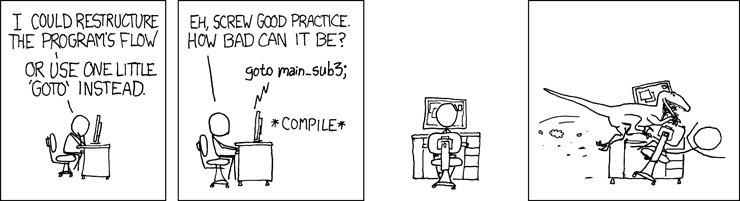
\includegraphics[height=1in,clip,trim=.65in 0 0 0]{pres_img/goto.png}\vspace{.2in}}
        \uncover<5->{
        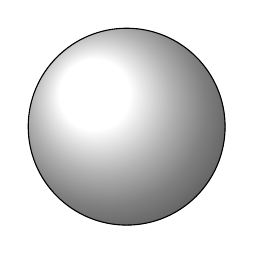
\begin{tikzpicture}
          \def\R{1.25} % sphere radius
          \def\angEl{35} % elevation angle
          \filldraw[ball color=white] (0,0) circle (\R);
          \foreach \t in {-80,-40,...,80} { \DrawLatitudeCircle[\R]{\t} }
          \foreach \t in {-5,-55,...,-175} { \DrawLongitudeCircle[\R]{\t}{black} }
          \DrawLongitudeCircle[\R]{-55}{red}
        \end{tikzpicture}}
      \end{columns}
    \end{frame}

    \begin{frame}{Putting it all together}
      \vspace{-.4in}
      \begin{columns}[T]
        \pause
        \column{0.5\textwidth}
        \vspace{.6in}
        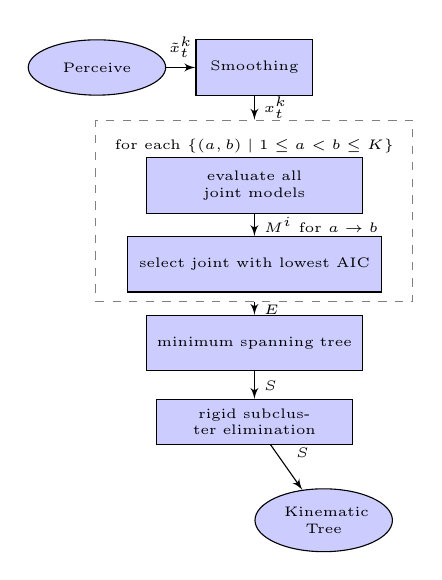
\begin{tikzpicture}[auto, >=latex']
          \tikzstyle{every node} = [font=\tiny]
          \tikzstyle{textbox} = [align=center, draw, fill=blue!20, minimum height=2em, minimum width=4em]
          \tikzstyle{block} = [textbox, ellipse]
          \tikzstyle{function} = [textbox, rectangle]
          \tikzstyle{pinstyle} = [pin edge={to-,thin,black}]

          \node (data) [block, text width=1cm] {Perceive};
          \node (preprocess) [function, right of=data, text width=1.25cm, node distance=2cm] {Smoothing};
          \node (foreach) [below of=preprocess, node distance=1cm] {for each $\{(a,b) \mid 1 \leq a < b \leq K\}$};
          \node (type) [function, below of=foreach, text width=2.5cm, node distance=.5cm] {evaluate all joint models};
          \node (bic) [function, below of=type, node distance=1cm, text width=3cm] {select joint with lowest AIC};
          \node (mst) [function, below of=bic, text width=2.5cm, node distance=1cm] {minimum spanning tree};
          \node (rigid) [function, below of=mst, text width=2.25cm, minimum height=.5cm, node distance=1cm] {rigid subcluster elimination};
          \node (tree) [block, below of=rigid, anchor=west, text width=1cm, node distance=1.25cm] {Kinematic\\Tree};

          \node (box) [draw=black!50, dashed, fit={(foreach) (type) (bic)}] {};
          \draw [->] (data) -- node {$\tilde{x}_t^k$} (preprocess);
          \draw [->] (preprocess) -- node {$x_t^k$} (box);
          \draw [->] (type) -- node {$\bowler{M}^i$ for $a \rightarrow b$} (bic);
          \draw [->] (box) -- node {$\bowler{E}$} (mst);
          \draw [->] (mst) -- node {$\bowler{S}$} (rigid);
          \draw [->] (rigid) -- node {$S$} (tree);
        \end{tikzpicture}

        \pause
        \column{0.5\textwidth}
        \tiny
        \begin{algorithm}[H]
          \SetFuncSty{textsc}
          \SetProcNameSty{textsc}
          \SetAlCapFnt{\scriptsize}
          \caption{\scriptsize Joint learner}
          \label{alg:manip-learn}
          \KwIn{$a,b$ tree edge, $\xse{x}_{1..T}^{a,b}$ object part positions}
          \KwOut{Joint $(J,\theta)$, states $\sigma_{1..T}$, cost $c$}
          \SetKwFunction{Optimize}{Min}
          \SetKwFunction{Rand}{Rnd}
          \SetKwFunction{FitPlane}{FitPlane}
          \SetKwFunction{Project}{Proj}
          \SetKwFunction{Unproject}{Unproj}
          \SetKwFunction{Circumcenter}{Circumcenter}
          \SetKw{KwInn}{in}
          \DontPrintSemicolon
          \BlankLine

          $\xse{\Delta}_{1..T} \leftarrow \xse{x}_{1..T}^b * (\xse{x}_{1..T}^a)^{-1}$ \;
          \For{$q$ \KwInn \{rigid, prismatic, revolute\}}{
          $i, j, k \leftarrow$ \Rand{$1..T$} \;
          \Switch{q}{
          \Case{rigid}{
          $\hat{\theta} \leftarrow \{\xse{\Delta}_i\}$ \;
          }
          \Case{prismatic}{
          $\hat{\theta} \leftarrow \{\xse{\Delta}_i, \frac{T^{-1}(\xse{\Delta}_k - \xse{\Delta}_i)}{||T^{-1}(\xse{\Delta}_k - \xse{\Delta}_i)||}\}$ \;
          }
          \Case{revolute}{
          $P \leftarrow$ \FitPlane{$T^{-1}(\xse{\Delta}_{1..T})$} \;
          $\xvec{\delta}_i, \xvec{\delta}_j, \xvec{\delta}_k \leftarrow$ \Project{$P$, $\xse{\Delta}_{\{i,j,k\}}$} \;
          $\xvec{c} \leftarrow$ \Unproject{$P$, \Circumcenter{$\xvec{\delta}_{\{i,j,k\}}$}} \\
          $\xse{c} \leftarrow T(\xvec{c})*\mat{c}{\xvec{P}_{d1} \\\hline \xvec{P}_{d2} \\\hline \xvec{P}_{d1} \times \xvec{P}_{d2}}$ \;
          $\hat{\theta} \leftarrow \{\xse{c}, \xse{\Delta}_i * \xse{c}^{-1}\}$ \;
          }
          }
          $(\theta_q, c_q) \leftarrow$ \Optimize{$\hat{\theta}$, $\lambda \theta .~ ||fk_q(\theta, ik_q(\xse{\Delta}, \theta)) - \xse{\Delta}||^2$}\; \label{line:optimize}
          }
          $J \leftarrow \displaystyle\min_q c_q$ \;
          $\sigma_{1..T} \leftarrow ik_J(\xse{\Delta}_{1..T}, \theta_J)$ \;
          \Return{$(J, \theta_J), \sigma_{1..T}, c_J$}
        \end{algorithm}
      \end{columns}
    \end{frame}

    \begin{frame}{Experiment 1: Simulation}
      \begin{columns}[t]
        \column{0.5\textwidth}
        \uncover<2->{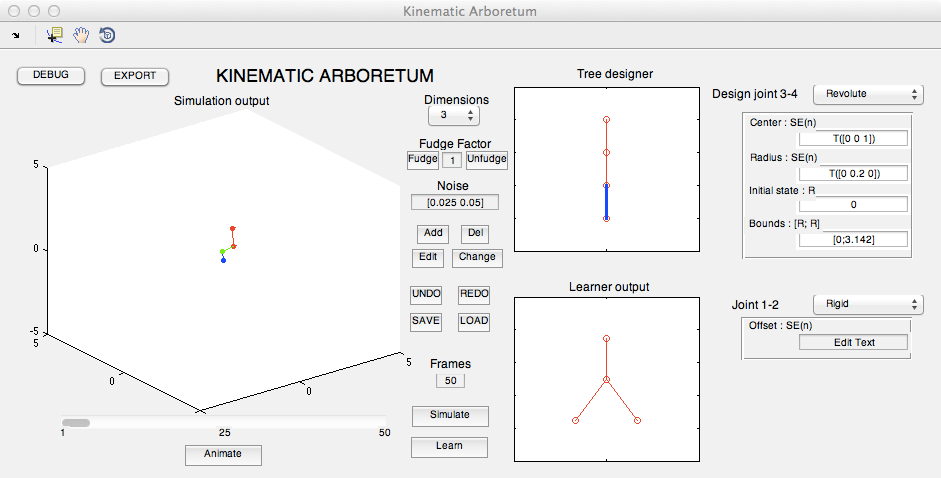
\includegraphics[width=\textwidth]{pres_img/screenshot.png}}
        \vspace{.05in}
        \uncover<5->{\begin{itemize}
          \item Main experiment: sensitivity of learning to noise and inflation
          \item Figure shows the simulation of a prismatic joint at three noise levels and the corresponding learning output
        \end{itemize}}

        \column{0.5\textwidth}
        \vspace{-1.1in}
        \uncover<3->{\begin{itemize}
          \item Tree designer GUI used to debug and experiment with simulation
          \item Control over simulation parameters: $T$, inflation, noise
        \end{itemize}}
        \vspace{.15in}
        \uncover<4->{\hspace{-.05\textwidth}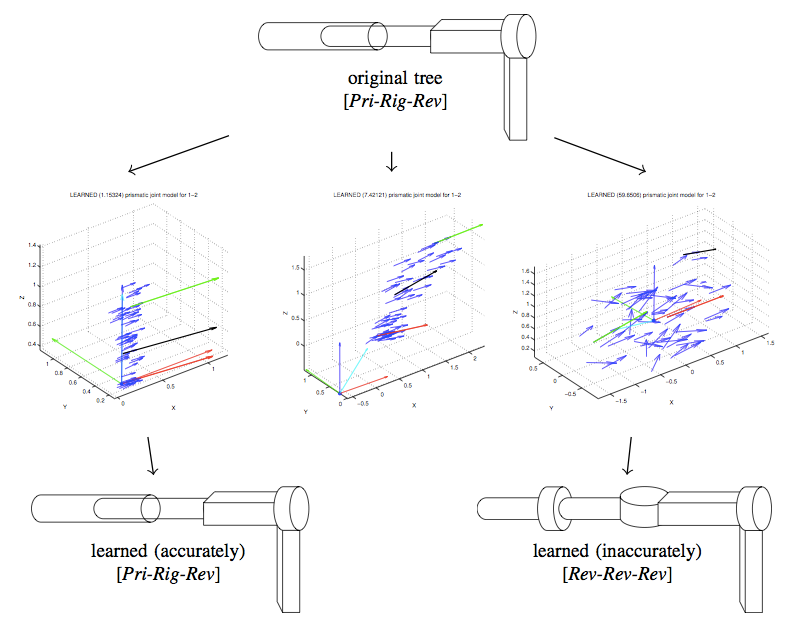
\includegraphics[width=1.1\textwidth]{pres_img/fig-exp1.png}}
      \end{columns}
    \end{frame}

    \begin{frame}{Experiment 2: Real World}
      \begin{columns}[t]
        \column{0.5\textwidth}
        \pause
        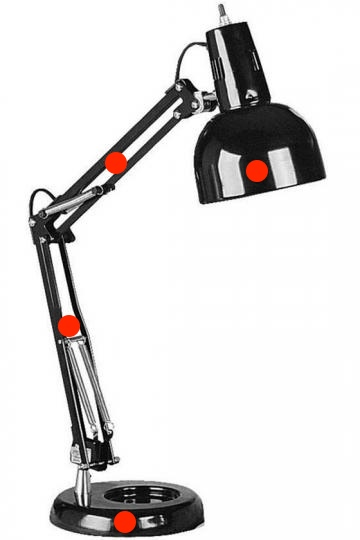
\includegraphics[width=.4\textwidth]{img/lamp.jpg}
        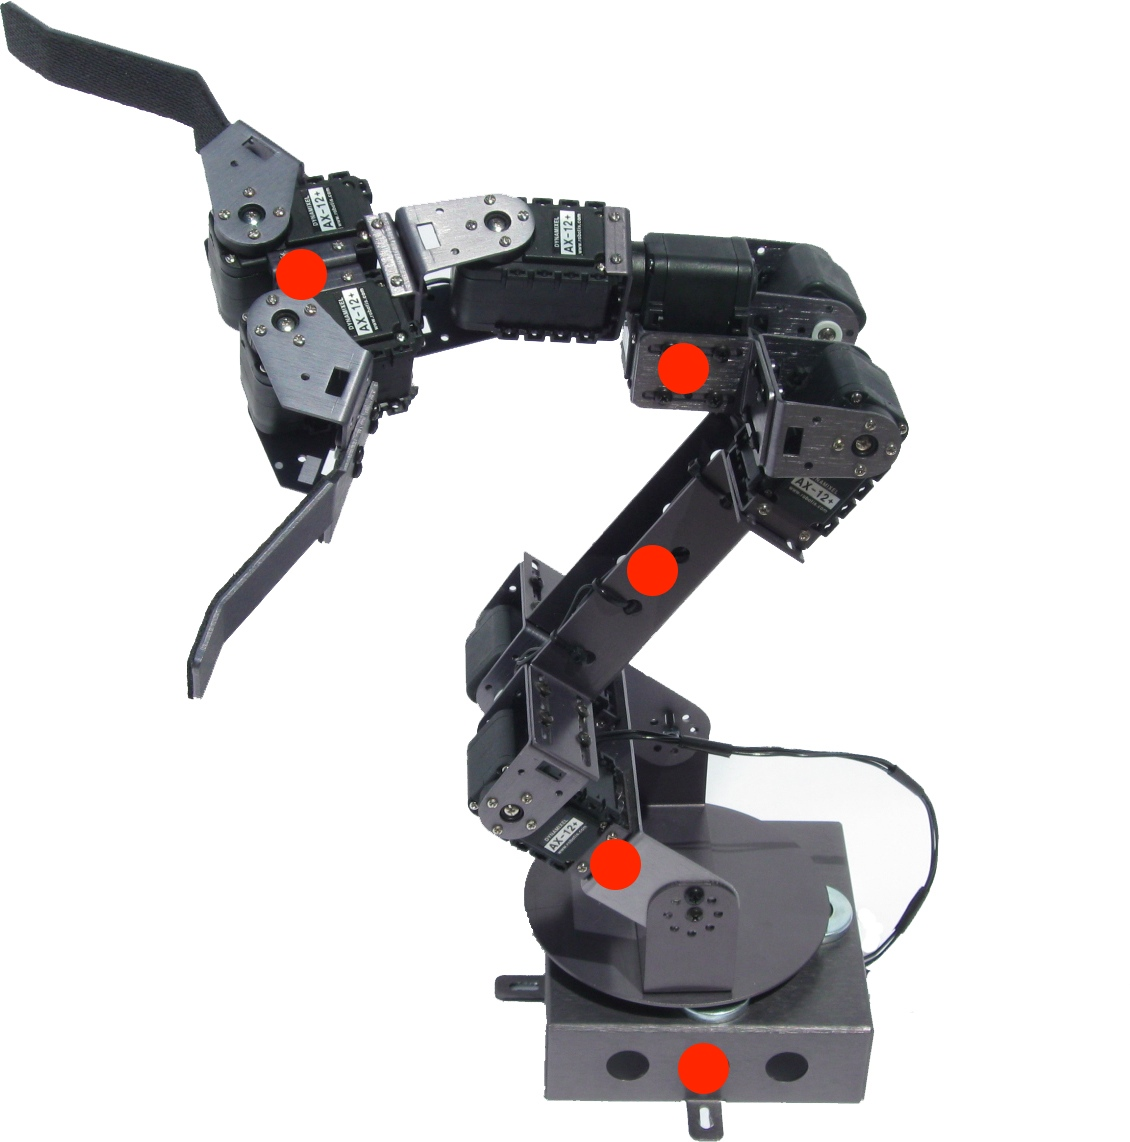
\includegraphics[width=.54\textwidth]{img/arm.jpg}
        \linebreak
        \linebreak
        \linebreak
        \pause
        \only<3>{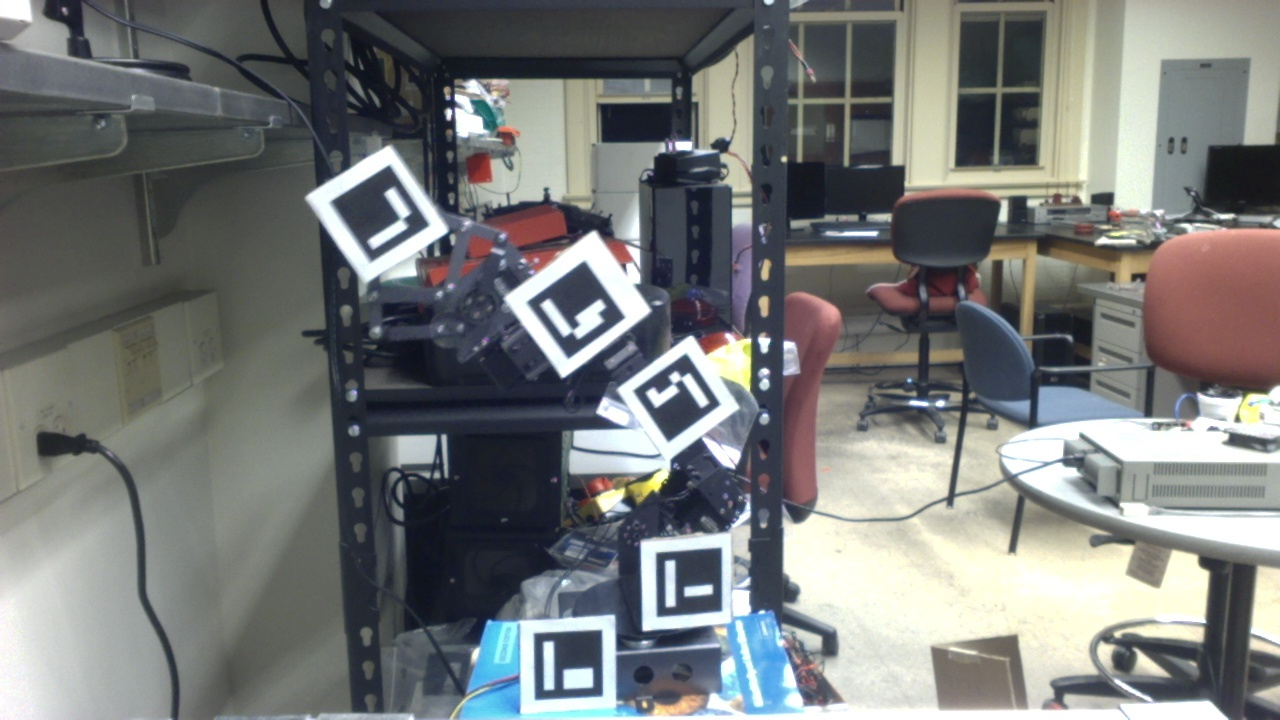
\includegraphics[width=\textwidth]{img/armdance_clean_343.jpg}}%
        \only<4->{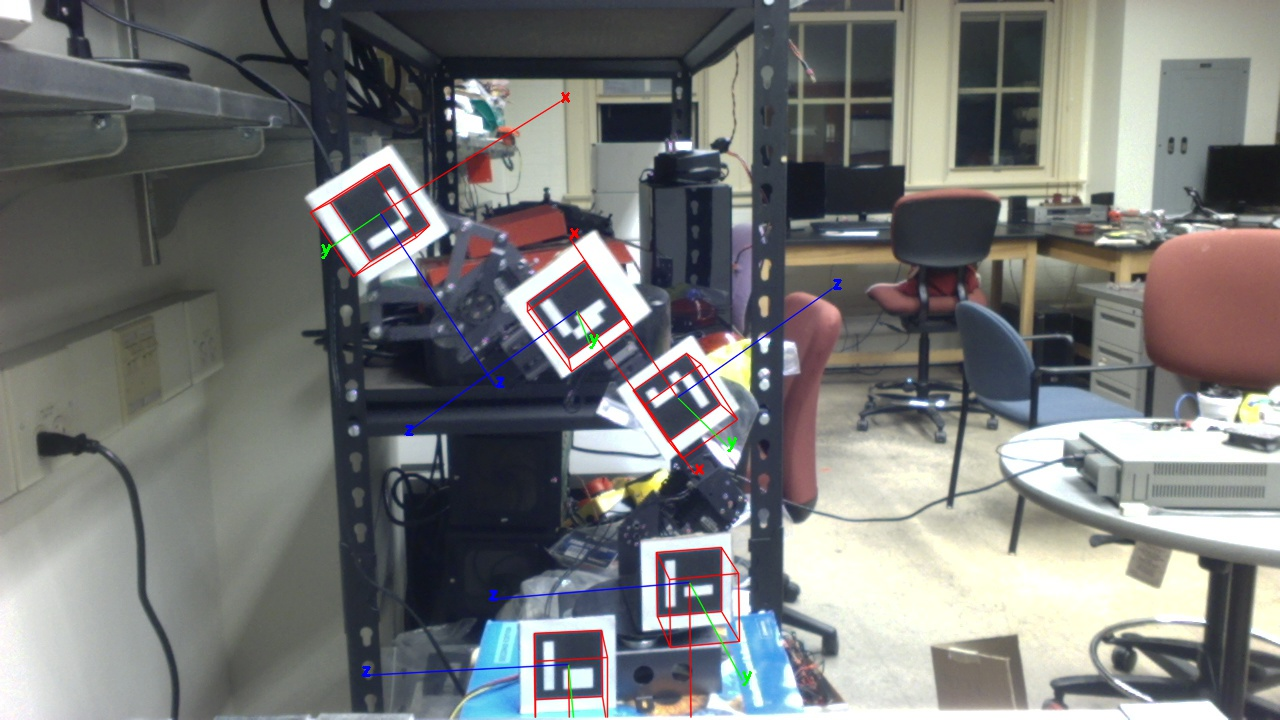
\includegraphics[width=\textwidth]{img/armdance_dirty_343.jpg}}

        \column{0.5\textwidth}
        \pause\pause
        \vspace{-1.3in}
        \begin{semiverbatim}
        \tiny
k shoulder -100 elbow -100 wrist 100 base -100

z 5

k base 75

z 5

k wrist 30

z 3

k wrist -60

z 3

k wrist 30

z 2

j

z 5
        \end{semiverbatim}
        \pause
        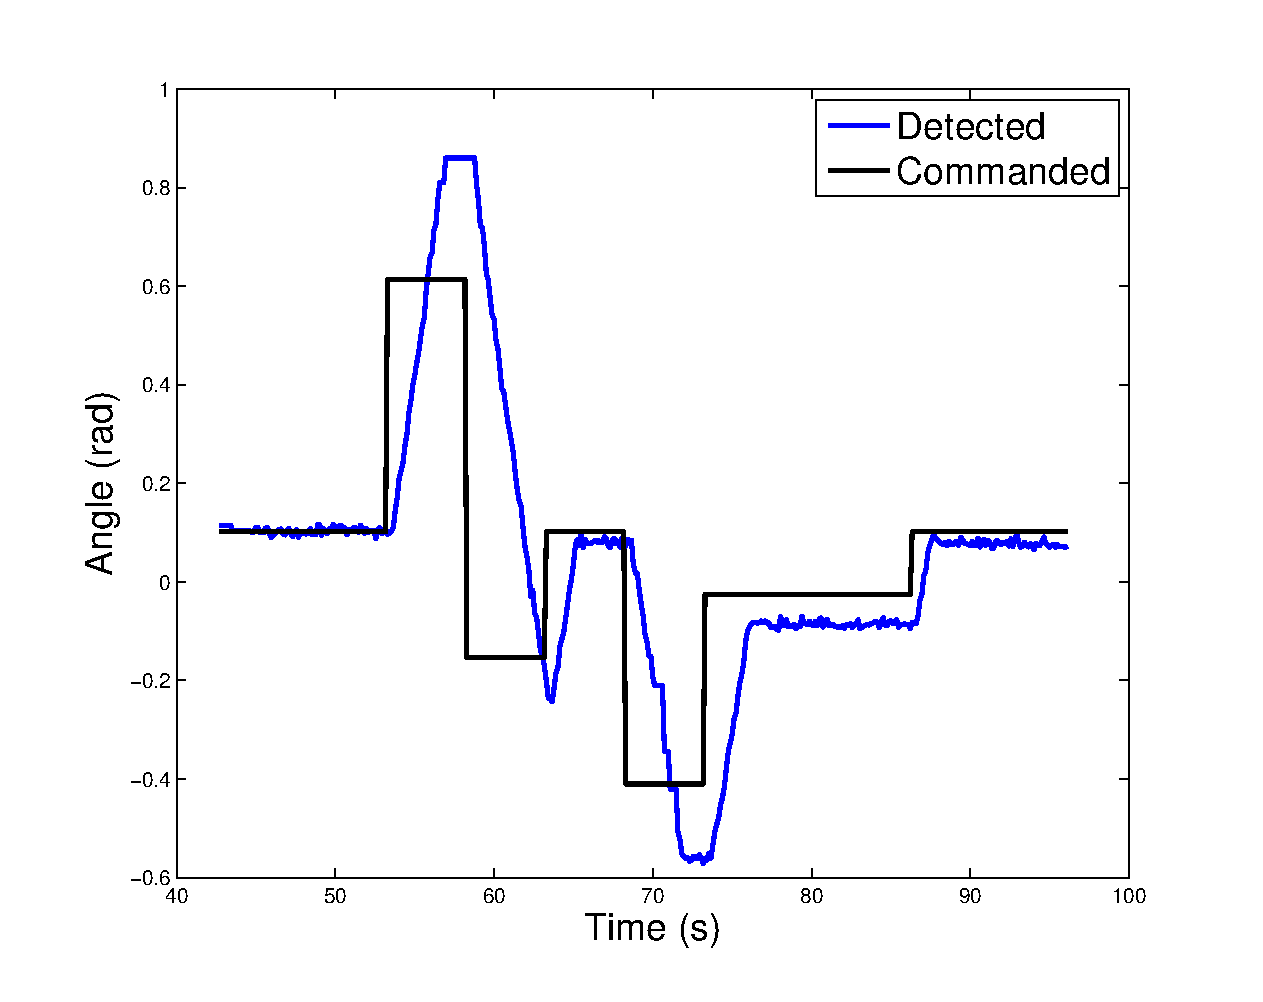
\includegraphics[width=\textwidth]{img/exp2b.eps}
      \end{columns}
    \end{frame}

\end{document}
